\ChapterImageStar[cap:disenio]{Diseño de la solución}{./images/fondo.png}\label{cap:disenio}
\mbox{}\\

El presente capítulo tiene como objetivo presentar una propuesta metodológica concreta para la definición de una notación unificada basada principalmente en ArchiMate aplicable en el contexto del programa de Ingeniería de Sistemas y Computación. En esta sección se especifica la estructura de la notación propuesta, detallando sus elementos seleccionados, capas definidas y reglas de representación que orientarán su uso en el área de Infraestructura de~\TI. Este diseño busca establecer las bases conceptuales para su implementación, promoviendo coherencia, claridad y sostenibilidad en la representación de la infraestructura tecnológica. Además, se pretende apoyar al grupo \GRID en el fortalecimiento de sus procesos formativos y en el cierre de las necesidades identificadas durante la caracterización.

La notación definida en este capítulo se fundamenta principalmente en la especificación oficial de ArchiMate, desarrollada por The Open Group. ArchiMate proporciona un lenguaje estandarizado para el modelado de arquitecturas empresariales, organizado por capas y con una semántica claramente definida.

A partir de esta base, la propuesta NDTI adopta los conceptos estructurales y relacionales que resultan pertinentes para el contexto académico del área de Infraestructura de TI. No obstante, con el fin de atender necesidades específicas identificadas en el programa, se realizan ajustes controlados en ciertos elementos gráficos y relaciones, así como la incorporación de nuevos símbolos que amplían la capacidad expresiva de la notación.

Estas extensiones no modifican la lógica conceptual central de ArchiMate, sino que la adaptan al entorno universitario, buscando mayor claridad pedagógica, simplificación semántica y alineación con los contenidos del plan curricular.

\section{Definición de capas}
\noindent
La notación propuesta en el marco del proyecto se organizará bajo un enfoque por capas, permitiendo representar la infraestructura de TI desde el nivel más concreto hasta el más abstracto, iniciando desde la capa física y culminando en la capa de negocio. . Esta estructura facilita la comprensión progresiva de los sistemas.

En este sentido, se definieron cuatro capas principales: Capa Física, Capa Tecnológica, Capa de Aplicación y Capa de Negocio.

\subsection{Capa Física}
\noindent
La Capa Física constituye el nivel base de la notación NDTI y representa los componentes materiales que soportan la infraestructura tecnológica. En esta capa se modelan los elementos tangibles que permiten la operación de los sistemas de información, incluyendo equipos, espacios físicos, redes de distribución y recursos materiales involucrados en la prestación de servicios tecnológicos.

Desde la perspectiva conceptual adoptada de ArchiMate, esta capa se fundamenta principalmente en elementos estructurales activos, pasivos y de conectividad pertenecientes a la capa tecnológica, manteniendo su semántica esencial pero orientándolos a su interpretación física. Esto permite representar de forma clara la infraestructura subyacente sobre la cual se construyen los demás niveles del modelo.

Desde la perspectiva conceptual adoptada de ArchiMate, esta capa se fundamenta principalmente en elementos estructurales activos, pasivos y de conectividad pertenecientes a la capa tecnológica, manteniendo su semántica esencial pero orientándolos a su interpretación física. Esto permite representar de forma clara la infraestructura subyacente sobre la cual se construyen los demás niveles del modelo.

De acuerdo a esto la especificación presentada a continuación define tanto los elementos adoptados directamente de ArchiMate como las extensiones propuestas en el proyecto NDTI, asegurando coherencia conceptual gráfica dentro del modelo.

\renewcommand{\arraystretch}{1.3}
\setlength{\extrarowheight}{2pt}
\fontsize{8.5pt}{10pt}\selectfont

\begin{longtable}{|
>{\centering\arraybackslash}m{1.8cm}|
>{\centering\arraybackslash}m{2.6cm}|
>{\centering\arraybackslash}m{2.1cm}|
>{\raggedright\arraybackslash}m{4.3cm}|
>{\centering\arraybackslash}m{2cm}|}

\caption{Especificación de elementos de la Capa Física en la notación NDTI}
\label{tab:capa_fisica_ndti} \\

\hline
\textbf{Ícono} & \textbf{Elemento} & \textbf{Clasificación} & \textbf{Descripción semántica} & \textbf{Origen} \\
\hline
\endfirsthead

\hline
\textbf{Ícono} & \textbf{Elemento} & \textbf{Clasificación} & \textbf{Descripción semántica} & \textbf{Origen} \\
\hline
\endhead

\hline
\endfoot

% ==========================================================
% ======== ELEMENTOS ADOPTADOS DE ARCHIMATE ===============
% ==========================================================

\hline
\multicolumn{5}{|c|}{\textbf{Elementos adoptados de ArchiMate}} \\
\hline


\includegraphics[width=1.1cm]{tablas-images/archi/fisica/archi_equipment.png}
& F-01 Componente (Activo)
& Estructural activo
& Máquina o recurso físico con capacidad de ejecutar comportamientos u operaciones dentro de la infraestructura.
& ArchiMate 3.x \\
\hline


\includegraphics[width=1.1cm]{tablas-images/archi/fisica/archi_facility.png}
& F-02 Locación
& Estructural activo
& Espacio físico destinado a alojar equipos e infraestructura tecnológica.
& ArchiMate 3.x \\
\hline


\includegraphics[width=1.1cm]{tablas-images/archi/fisica/archi_dn.png}
& F-03 Red de distribución
& Conectividad
& Infraestructura física que permite el transporte o suministro de recursos entre distintos puntos. En la notación, este elemento incorpora una etiqueta descriptiva que identifica el tipo de red de distribución representada (por ejemplo, datos, energía, insumos, entre otros), facilitando su diferenciación semántica dentro del modelo.
& ArchiMate 3.x \\
\hline


\includegraphics[width=1.1cm]{tablas-images/archi/fisica/archi_material.png} 
& F-04 Material 
& Estructural pasivo 
& Elemento físico susceptible de ser utilizado, transformado o consumido dentro de un proceso. 
& ArchiMate 3.x \\ 
\hline

% ==========================================================
% ======== EXTENSIONES PROPUESTAS EN NDTI ==================
% ==========================================================

\hline
\multicolumn{5}{|c|}{\textbf{Extensiones propuestas por el proyecto}} \\
\hline


\includegraphics[width=1.1cm]{tablas-images/archi/fisica/nditi_pascomp.png}
& F-05 Componente (Pasivo)
& Estructural pasivo
& Elemento físico susceptible de ser utilizado, transformado o consumido dentro de un proceso.
& Propuesta NDTI \\
\hline

\end{longtable}

\subsubsection{Capa de Redes y Comunicaciones}
\noindent

La Capa de Redes y Comunicaciones se introduce en la notación NDTI como una extensión orientada a representar de manera más detallada y estructurada los elementos asociados a la conectividad dentro de la infraestructura de TI. Aunque ArchiMate contempla conceptos generales de red y comunicación, no proporciona un conjunto de elementos suficientemente específico para modelar dispositivos y componentes comúnmente utilizados en el contexto académico del área de Infraestructura de TI.

Con el propósito de cubrir esta limitación, se define una capa especializada que agrupa elementos propios del dominio de redes y comunicaciones, tales como dispositivos de interconexión, nodos de conexión y equipos asociados a la transmisión y gestión del tráfico de datos. Estos elementos se plantean como especializaciones físicas del concepto general de equipo o como nuevas abstracciones necesarias para representar adecuadamente la topología y organización de una red.

La Capa de Redes y Comunicaciones se introduce en la notación NDTI como una extensión orientada a representar de manera más detallada y estructurada los elementos asociados a la conectividad dentro de la infraestructura de TI. Aunque ArchiMate contempla conceptos generales de red y comunicación, no proporciona un conjunto de elementos suficientemente específico para modelar dispositivos y componentes comúnmente utilizados en el contexto académico del área de Infraestructura de TI.

Con el propósito de cubrir esta limitación, se define una capa especializada que agrupa elementos propios del dominio de redes y comunicaciones, tales como dispositivos de interconexión, nodos de conexión y equipos asociados a la transmisión y gestión del tráfico de datos. Estos elementos se plantean como especializaciones físicas del concepto general de equipo o como nuevas abstracciones necesarias para representar adecuadamente la topología y organización de una red.

La separación de estos componentes en una capa independiente permite mejorar la claridad del modelo, facilitando la lectura, el análisis y la enseñanza de arquitecturas de red dentro del programa. Asimismo, esta organización favorece un uso más estructurado de la notación, alineado con las necesidades específicas de asignaturas relacionadas con redes, comunicaciones e infraestructura tecnológica.

\begin{longtable}{|
>{\centering\arraybackslash}m{1.8cm}|
>{\centering\arraybackslash}m{2.6cm}|
>{\centering\arraybackslash}m{2.1cm}|
>{\raggedright\arraybackslash}m{4.3cm}|
>{\centering\arraybackslash}m{2cm}|}

\caption{Especificación de elementos de la Capa de Redes y Comunicaciones en la notación NDTI}
\label{tab:capa_ryc_ndti} \\

\hline
\textbf{Ícono} & \textbf{Elemento} & \textbf{Clasificación} & \textbf{Descripción semántica} & \textbf{Origen} \\
\hline
\endfirsthead

\hline
\textbf{Ícono} & \textbf{Elemento} & \textbf{Clasificación} & \textbf{Descripción semántica} & \textbf{Origen} \\
\hline
\endhead

\hline
\endfoot

% ==========================================================
% ======== EXTENSIONES PROPUESTAS EN NDTI ==================
% ==========================================================

\hline
\multicolumn{5}{|c|}{\textbf{Extensiones propuestas por el proyecto}} \\
\hline


\includegraphics[width=1.1cm]{tablas-images/archi/redes_comunicaciones/nditi_node.png}
& RC-01 Nodo de conexión
& Estructural activo
& Punto físico de interconexión dentro de una red de distribución que permite enlazar, concentrar o derivar conexiones entre múltiples dispositivos, equipos o segmentos de red. Puede representar puntos de acceso, panes de conexión (\textit{patch panels}), concentradores físicos, etc.
& Google Fonts \\
\hline


\includegraphics[width=1.1cm]{tablas-images/archi/redes_comunicaciones/nditi_router.png}
& RC-02 Router
& Especialización física de Equipo
& Dispositivo físico de interconexión de redes encargado de dirigir el tráfico de datos entre diferentes segmentos de red.
& Freepik \\
\hline

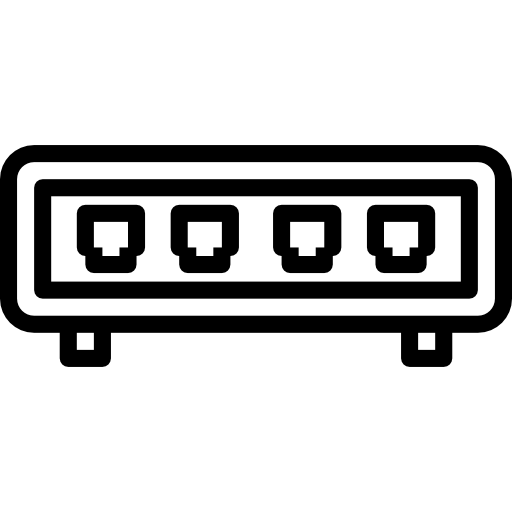
\includegraphics[width=1.1cm]{tablas-images/archi/redes_comunicaciones/nditi_switch.png}
& RC-03 Switch
& Especialización física de Equipo
& Dispositivo físico que permite la interconexión de múltiples dispositivos dentro de una red local, gestionando el tráfico mediante direcciones físicas.
& Freepik \\
\hline


\includegraphics[width=1.1cm]{tablas-images/archi/redes_comunicaciones/nditi_server.png}
& RC-04 Servidor (Hardware)
& Especialización física de Equipo
& Equipo físico de alto desempeño destinado a proporcionar recursos computacionales, almacenamiento o servicios a otros dispositivos.
& Freepik \\
\hline


\includegraphics[width=1.1cm]{tablas-images/archi/redes_comunicaciones/nditi_modem.png}
& RC-05 Módem
& Especialización física de Equipo
& Dispositivo físico encargado de modular y demodular señales para permitir la transmisión de datos a través de medios de comunicación externos.
& Freepik \\
\hline


\includegraphics[width=1.1cm]{tablas-images/archi/redes_comunicaciones/nditi_firewall.png}
& RC-06 Firewall físico
& Especialización física de Equipo
& Dispositivo físico de seguridad de red que controla y filtra el tráfico de datos según políticas predefinidas.
& Google Fonts \\
\hline


\includegraphics[width=1.1cm]{tablas-images/archi/redes_comunicaciones/nditi_disk.png}
& RC-07 Dispositivo de almacenamiento físico
& Especialización física de Equipo
& Equipo físico destinado al almacenamiento persistente de información, tales como sistemas NAS, SAN o arreglos de discos.
& Google Fonts \\
\hline


\includegraphics[width=1.1cm]{tablas-images/archi/fisica/nditi_generic.png}
& RC-08 Dispositivo genérico físico
& Especialización física de Equipo
& Elemento físico no especificado utilizado para representar cualquier dispositivo de infraestructura tecnológica cuya naturaleza particular no se detalla en el modelo.
& Google Fonts \\

\end{longtable}



\subsubsection{Capa Tecnológica}
\noindent

La Capa Tecnológica en la notación NDTI representa el nivel en el que se abstraen los recursos computacionales y los servicios que soportan la ejecución de software dentro de la infraestructura de TI. A diferencia de la capa física, en este nivel se modelan los componentes lógicos, los entornos de ejecución y los comportamientos tecnológicos que permiten la operación de los sistemas.

Esta capa se fundamenta directamente en la especificación de ArchiMate, adoptando sus principales elementos estructurales, de conectividad y de comportamiento, tales como nodos, software de sistema, servicios tecnológicos y procesos. Estos elementos proporcionan una base sólida y estandarizada para la representación de arquitecturas tecnológicas. No obstante, a partir de las necesidades identificadas en el contexto académico del programa, se incorporan extensiones específicas que permiten representar conceptos actuales ampliamente utilizados en la industria, como la virtualización y la contenedorización. Elementos como el nodo servidor, las máquinas virtuales, los contenedores de software y los mecanismos de seguridad lógica amplían la capacidad expresiva de la notación, facilitando la modelación de escenarios reales abordados en asignaturas del área de Infraestructura de TI.

De esta manera, la capa tecnológica integra tanto los elementos propios de ArchiMate como las extensiones propuestas en el proyecto NDTI, manteniendo la coherencia conceptual.

\begin{longtable}{|
>{\centering\arraybackslash}m{1.8cm}|
>{\centering\arraybackslash}m{2.6cm}|
>{\centering\arraybackslash}m{2.1cm}|
>{\raggedright\arraybackslash}m{4.3cm}|
>{\centering\arraybackslash}m{2cm}|}

\caption{Especificación de elementos de la Capa Física en la notación NDTI}
\label{tab:capa_tecnologica_ndti} \\

\hline
\textbf{Ícono} & \textbf{Elemento} & \textbf{Clasificación} & \textbf{Descripción semántica} & \textbf{Origen} \\
\hline
\endfirsthead

\hline
\textbf{Ícono} & \textbf{Elemento} & \textbf{Clasificación} & \textbf{Descripción semántica} & \textbf{Origen} \\
\hline
\endhead

\hline
\endfoot

% ==========================================================
% ======== ELEMENTOS ADOPTADOS DE ARCHIMATE ===============
% ==========================================================

\hline
\multicolumn{5}{|c|}{\textbf{Elementos adoptados de ArchiMate}} \\
\hline

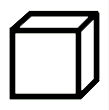
\includegraphics[width=1.1cm]{tablas-images/archi/tec/archi_node.png}
& T-01 Nodo
& Estructural activo
& Recurso computacional capaz de ejecutar artefactos de software y alojar otros elementos tecnológicos dentro de la infraestructura.
& ArchiMate 3.x \\
\hline


\includegraphics[width=1.1cm]{tablas-images/archi/tec/archi_device.png}
& T-02 Dispositivo
& Estructural activo
& Componente físico de hardware que proporciona capacidad de procesamiento, almacenamiento o conectividad.
& ArchiMate 3.x \\
\hline


\includegraphics[width=1.1cm]{tablas-images/archi/tec/archi_syssoft.png}
& T-03 Software de Sistema
& Estructural activo
& Software base que gestiona los recursos del hardware y provee servicios fundamentales para la ejecución de aplicaciones.
& ArchiMate 3.x \\
\hline

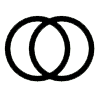
\includegraphics[width=1.1cm]{tablas-images/archi/tec/archi_techco.png}
& T-04 Colaboración Tecnológica
& Estructural activo
& Agrupación de nodos o recursos tecnológicos que cooperan para ofrecer una capacidad conjunta.
& ArchiMate 3.x \\
\hline

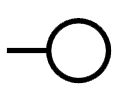
\includegraphics[width=1.1cm]{tablas-images/archi/tec/archi_techin.png}
& T-05 Interfaz Tecnológica
& Estructural activo
& Punto de acceso a través del cual se exponen servicios o funcionalidades tecnológicas a otros elementos.
& ArchiMate 3.x \\
\hline

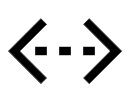
\includegraphics[width=1.1cm]{tablas-images/archi/tec/archi_path.png}
& T-06 Camino
& Conectividad
& Canal lógico o físico que permite la comunicación entre nodos o dispositivos dentro de la infraestructura.
& ArchiMate 3.x \\
\hline

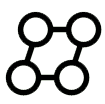
\includegraphics[width=1.1cm]{tablas-images/archi/tec/archi_comnet.png}
& T-07 Red de Comunicación
& Conectividad
& Infraestructura de red que posibilita la transmisión estructurada de datos entre múltiples elementos tecnológicos.
& ArchiMate 3.x \\
\hline


\includegraphics[width=1.1cm]{tablas-images/archi/tec/archi_techfunc.png}
& T-08 Función Tecnológica
& Conductual
& Comportamiento interno automatizado que describe capacidades ejecutadas por un nodo o sistema.
& ArchiMate 3.x \\
\hline



\includegraphics[width=1.1cm]{tablas-images/archi/tec/archi_techpro.png}
& T-09 Proceso Tecnológico
& Conductual
& Secuencia organizada de actividades técnicas orientadas a cumplir un objetivo operativo específico.
& ArchiMate 3.x \\
\hline


\includegraphics[width=1.1cm]{tablas-images/archi/tec/archi_techint.png}
& T-10 Interacción Tecnológica
& Conductual
& Comportamiento colaborativo entre múltiples nodos o sistemas para ejecutar una función conjunta.
& ArchiMate 3.x \\
\hline

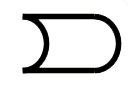
\includegraphics[width=1.1cm]{tablas-images/archi/tec/archi_techevent.png}
& T-11 Evento Tecnológico
& Conductual
& Suceso identificable que desencadena o modifica el comportamiento de elementos tecnológicos.
& ArchiMate 3.x \\
\hline


\includegraphics[width=1.1cm]{tablas-images/archi/tec/archi_techserv.png}
& T-12 Servicio Tecnológico
& Conductual (Externo)
& Capacidad tecnológica expuesta a otras capas como un servicio consumible.
& ArchiMate 3.x \\
\hline


\includegraphics[width=1.1cm]{tablas-images/archi/tec/archi_arti.png}
& T-13 Artefacto
& Estructural pasivo
& Objeto digital que es producido, utilizado o desplegado por elementos tecnológicos.
& ArchiMate 3.x \\
\hline

% ==========================================================
% ======== EXTENSIONES PROPUESTAS EN NDTI ==================
% ==========================================================

\hline
\multicolumn{5}{|c|}{\textbf{Extensiones propuestas por el proyecto}} \\
\hline


\includegraphics[width=1.1cm]{tablas-images/archi/tec/nditi_lserver.png}
& T-14 Nodo servidor
& Estructural activo
& Entorno lógico de ejecución asociado a recursos computacionales dentro de la infraestructura tecnológica. Representa instancias de servidor que operan sobre infraestructura física o virtualizada, tales como máquinas virtuales o contenedores.
& Google Fonts \\
\hline


\includegraphics[width=1.1cm]{tablas-images/archi/tec/nditi_container.png}
& T-15 Contenedor de software
& Estructural activo
& Entorno de ejecución ligero y aislado que encapsula aplicaciones y sus dependencias, permitiendo su despliegue consistente sobre una infraestructura compartida. Este elemento representa tecnologías de contenedorización como Docker y se ubica sobre nodos servidores o plataformas de virtualización, facilitando la portabilidad y escalabilidad de los sistemas.
& Google Fonts \\
\hline


\includegraphics[width=1.1cm]{tablas-images/archi/tec/nditi_vm.png}
& T-16 Máquina Virtual
& Estructural activo
& Entorno de ejecución virtualizado que opera sobre un servidor físico o plataforma de virtualización, permitiendo la ejecución aislada de sistemas operativos y aplicaciones dentro de la infraestructura tecnológica.
& Google Fonts \\
\hline


\includegraphics[width=1.1cm]{tablas-images/archi/tec/nditi_lofw.png}
& T-17 Firewall lógico
& Estructural activo
& Mecanismo de seguridad implementado mediante software que controla y filtra el tráfico de red entre diferentes componentes de la infraestructura tecnológica según reglas de seguridad definidas.
& Google Fonts \\
\hline

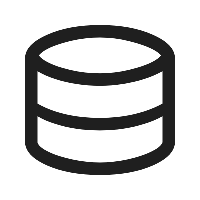
\includegraphics[width=1.1cm]{tablas-images/archi/tec/nditi_db.png}
& T-18 Servicio de almacenamiento
& Conductual (externo)
& Servicio tecnológico encargado de proporcionar capacidades de almacenamiento y gestión de datos a otros componentes de la infraestructura o a capas superiores del modelo.
& Google Fonts \\
\hline


\end{longtable}

\subsubsection{Capa de Aplicación}
\noindent

La Capa de Aplicación en la notación NDTI representa el nivel en el que se modelan los sistemas de software y sus funcionalidades desde una perspectiva lógica. En esta capa se describen los componentes de aplicación, sus interacciones, los procesos que ejecutan y los datos que gestionan, permitiendo abstraer la lógica del sistema independientemente de la infraestructura tecnológica subyacente.

Esta capa se fundamenta en los elementos definidos por ArchiMate para el modelado de aplicaciones, adoptando sus conceptos estructurales, conductuales y pasivos, tales como componentes de aplicación, interfaces, servicios, procesos, eventos y objetos de datos. Estos elementos proporcionan una base sólida y estandarizada para representar la arquitectura de software dentro de un sistema. Adicionalmente, con el fin de mejorar la capacidad expresiva de la notación, se incorporan extensiones específicas orientadas a la comprensión de arquitecturas modernas y al proceso de enseñanza. Entre estas extensiones se incluyen elementos auxiliares como restricciones y notas, que permiten complementar la semántica del modelo, así como elementos estructurales como el nodo funcional, que facilita la descomposición interna de los componentes de aplicación.

Adicionalmente, se introduce el concepto de API o Gateway de aplicación, el cual permite representar de forma explícita los puntos de exposición de servicios en arquitecturas basadas en APIs, y el orquestador de aplicación, que modela la coordinación de flujos entre múltiples componentes. Estas incorporaciones buscan acercar la notación a escenarios reales de desarrollo de software, manteniendo al mismo tiempo coherencia con la estructura conceptual de ArchiMate.

De esta manera, la capa de aplicación integra tanto los elementos propios del estándar como las extensiones propuestas en el proyecto NDTI, permitiendo una representación clara, consistente y alineada con las necesidades del programa en el área de Infraestructura de TI.

\renewcommand{\arraystretch}{1.3}
\setlength{\extrarowheight}{2pt}
\fontsize{8.5pt}{10pt}\selectfont

\begin{longtable}{|
>{\centering\arraybackslash}m{1.8cm}|
>{\centering\arraybackslash}m{2.6cm}|
>{\centering\arraybackslash}m{2.1cm}|
>{\raggedright\arraybackslash}m{4.3cm}|
>{\centering\arraybackslash}m{2cm}|}

\caption{Especificación de elementos de la Capa de Aplicación en la notación NDTI}
\label{tab:capa_aplicacion_ndti} \\

\hline
\textbf{Ícono} & \textbf{Elemento} & \textbf{Clasificación} & \textbf{Descripción semántica} & \textbf{Origen} \\
\hline
\endfirsthead

\hline
\textbf{Ícono} & \textbf{Elemento} & \textbf{Clasificación} & \textbf{Descripción semántica} & \textbf{Origen} \\
\hline
\endhead

\hline
\endfoot

% ==========================================================
% ======== ELEMENTOS ADOPTADOS DE ARCHIMATE ===============
% ==========================================================

\hline
\multicolumn{5}{|c|}{\textbf{Elementos adoptados de ArchiMate}} \\
\hline


\includegraphics[width=1.1cm]{tablas-images/archi/app/archi_appcomp.png}
& A-01 Componente de Aplicación
& Estructural activo
& Unidad modular de software que encapsula funcionalidad y datos dentro de un sistema.
& ArchiMate 3.x \\
\hline

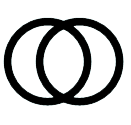
\includegraphics[width=1.1cm]{tablas-images/archi/app/archi_appcollab.png}
& A-02 Colaboración de Aplicación
& Estructural activo
& Conjunto de componentes de aplicación que trabajan de manera conjunta para ofrecer una funcionalidad integrada.
& ArchiMate 3.x \\
\hline

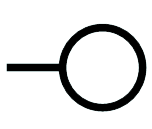
\includegraphics[width=1.1cm]{tablas-images/archi/app/archi_appinterface.png}
& A-03 Interfaz de Aplicación
& Estructural activo
& Punto de acceso a través del cual un componente de aplicación expone su funcionalidad.
& ArchiMate 3.x \\
\hline


\includegraphics[width=1.1cm]{tablas-images/archi/app/archi_appfunc.png}
& A-04 Función de Aplicación
& Conductual
& Comportamiento interno automatizado que describe capacidades ejecutadas por un componente de aplicación.
& ArchiMate 3.x \\
\hline


\includegraphics[width=1.1cm]{tablas-images/archi/app/archi_appinteract.png}
& A-05 Interacción de Aplicación
& Conductual
& Comportamiento colaborativo entre múltiples componentes de aplicación.
& ArchiMate 3.x \\
\hline

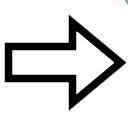
\includegraphics[width=1.1cm]{tablas-images/archi/app/archi_appproc.png}
& A-06 Proceso de Aplicación
& Conductual
& Secuencia estructurada de actividades ejecutadas por uno o varios componentes de aplicación.
& ArchiMate 3.x \\
\hline

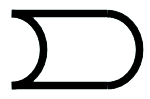
\includegraphics[width=1.1cm]{tablas-images/archi/app/archi_appevent.png}
& A-07 Evento de Aplicación
& Conductual
& Suceso que desencadena o modifica el comportamiento dentro de la aplicación.
& ArchiMate 3.x \\
\hline


\includegraphics[width=1.1cm]{tablas-images/archi/app/archi_appservice.png}
& A-08 Servicio de Aplicación
& Conductual (externo)
& Funcionalidad expuesta por la aplicación para ser consumida por otras capas o sistemas.
& ArchiMate 3.x \\
\hline

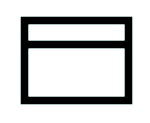
\includegraphics[width=1.1cm]{tablas-images/archi/app/archi_dataobj.png}
& A-09 Objeto de Datos
& Estructural pasivo
& Representación de datos utilizados o producidos por componentes de aplicación.
& ArchiMate 3.x \\
\hline

% ==========================================================
% ======== EXTENSIONES PROPUESTAS EN NDTI ==================
% ==========================================================

\hline
\multicolumn{5}{|c|}{\textbf{Extensiones propuestas por el proyecto}} \\
\hline

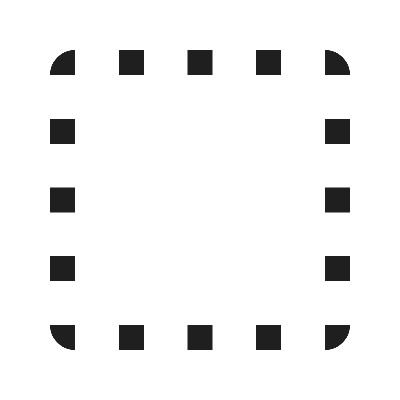
\includegraphics[width=1.1cm]{tablas-images/archi/app/ndti_constraint.png}
& A-10 Restricción
& Elemento auxiliar
& Elemento que permite representar condiciones, reglas o limitaciones que afectan el comportamiento o la estructura de los componentes de aplicación. Se utiliza para complementar la semántica del modelo sin representar un componente ejecutable.
& Google Fonts \\
\hline


\includegraphics[width=1.1cm]{tablas-images/archi/app/ndti_note.png}
& A-11 Nota
& Elemento auxiliar
& Elemento textual utilizado para añadir aclaraciones, comentarios o información adicional dentro del modelo, facilitando su comprensión sin alterar la semántica de los elementos principales.
& Google Fonts \\
\hline


\includegraphics[width=1.1cm]{tablas-images/archi/app/ndti_functional_node.png}
& A-12 Nodo funcional
& Elemento estructural
& Elemento gráfico utilizado para subdividir un componente de aplicación en unidades internas que representan funcionalidades específicas, permitiendo una descomposición más detallada del comportamiento del sistema.
& Google Fonts \\
\hline


\includegraphics[width=1.1cm]{tablas-images/archi/app/ndti_api_gateway.png}
& A-13 API / Gateway de Aplicación
& Estructural activo
& Componente de aplicación que centraliza la exposición de servicios a través de interfaces unificadas, gestionando aspectos como enrutamiento, autenticación, control de acceso y agregación de respuestas. Se modela como una especialización de la interfaz de aplicación, facilitando la representación de arquitecturas basadas en APIs.
& Google Fonts \\
\hline


\includegraphics[width=1.1cm]{tablas-images/archi/app/ndti_orchestrator.png}
& A-14 Orquestador de Aplicación
& Conductual
& Elemento encargado de coordinar la ejecución de múltiples componentes o servicios de aplicación, definiendo el flujo de interacción entre ellos para cumplir un objetivo funcional específico. Permite representar patrones de orquestación en arquitecturas distribuidas.
& Google Fonts \\
\hline

\end{longtable}


\subsubsection{Capa de Negocio}
\noindent

La Capa de Negocio representa el nivel más abstracto de la notación NDTI y tiene como propósito modelar los elementos organizacionales, los procesos y la lógica operativa que dan sentido a la infraestructura tecnológica. En esta capa se describen los actores, roles, servicios y objetos de negocio, así como las interacciones y comportamientos que permiten la generación de valor dentro de un contexto organizacional.

Desde el punto de vista conceptual, esta capa se fundamenta en los elementos definidos por ArchiMate para el modelado del dominio de negocio, manteniendo su semántica original y su estructura basada en elementos estructurales, conductuales y pasivos. Esto permite representar de manera coherente la relación entre los procesos de negocio y las capas inferiores de la arquitectura.

No obstante, a partir del análisis de las necesidades del programa académico, se identificó la necesidad de complementar esta capa con elementos adicionales orientados a la representación explícita de flujos de proceso. En este sentido, la propuesta NDTI incorpora un conjunto de extensiones inspiradas en notaciones como BPMN y diagramas de actividades, las cuales permiten modelar de manera más clara aspectos como el inicio y fin de procesos, decisiones, paralelización, ciclos y organización por responsabilidades.

Estas extensiones no sustituyen los elementos propios de ArchiMate, sino que actúan como un complemento visual y semántico que facilita la comprensión de los procesos de negocio, especialmente en contextos educativos. De esta manera, la Capa de Negocio en NDTI logra integrar la solidez estructural de ArchiMate con la expresividad de las notaciones de flujo, proporcionando una representación más completa, intuitiva y alineada con los objetivos formativos del área de Infraestructura de TI.

\renewcommand{\arraystretch}{1.3}
\setlength{\extrarowheight}{2pt}
\fontsize{8.5pt}{10pt}\selectfont

\begin{longtable}{|
>{\centering\arraybackslash}m{1.8cm}|
>{\centering\arraybackslash}m{2.6cm}|
>{\centering\arraybackslash}m{2.1cm}|
>{\raggedright\arraybackslash}m{4.3cm}|
>{\centering\arraybackslash}m{2cm}|}

\caption{Especificación de elementos de la Capa de Negocio en la notación NDTI}
\label{tab:capa_negocio_ndti} \\

\hline
\textbf{Ícono} & \textbf{Elemento} & \textbf{Clasificación} & \textbf{Descripción semántica} & \textbf{Origen} \\
\hline
\endfirsthead

\hline
\textbf{Ícono} & \textbf{Elemento} & \textbf{Clasificación} & \textbf{Descripción semántica} & \textbf{Origen} \\
\hline
\endhead

\hline
\endfoot

% ==========================================================
% ======== ELEMENTOS ADOPTADOS DE ARCHIMATE ===============
% ==========================================================

\hline
\multicolumn{5}{|c|}{\textbf{Elementos adoptados de ArchiMate}} \\
\hline


\includegraphics[width=1.1cm]{tablas-images/archi/business/archi_actor.png}
& B-01 Actor de Negocio
& Estructural activo
& Entidad que realiza comportamientos dentro del negocio, pudiendo corresponder a una persona, organización o sistema.
& ArchiMate 3.x \\
\hline

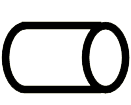
\includegraphics[width=1.1cm]{tablas-images/archi/business/archi_role.png}
& B-02 Rol de Negocio
& Estructural activo
& Responsabilidad o función asumida por un actor dentro de un contexto organizacional específico.
& ArchiMate 3.x \\
\hline

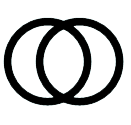
\includegraphics[width=1.1cm]{tablas-images/archi/business/archi_collab.png}
& B-03 Colaboración de Negocio
& Estructural activo
& Conjunto de actores o roles que cooperan para alcanzar un objetivo común dentro del negocio.
& ArchiMate 3.x \\
\hline

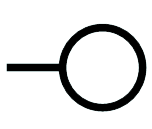
\includegraphics[width=1.1cm]{tablas-images/archi/business/archi_interface.png}
& B-04 Interfaz de Negocio
& Estructural activo
& Punto de acceso mediante el cual un actor o rol expone servicios hacia otros actores o al entorno.
& ArchiMate 3.x \\
\hline

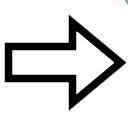
\includegraphics[width=1.1cm]{tablas-images/archi/business/archi_process.png}
& B-05 Proceso de Negocio
& Conductual
& Secuencia estructurada de actividades que se ejecutan para cumplir un objetivo del negocio.
& ArchiMate 3.x \\
\hline


\includegraphics[width=1.1cm]{tablas-images/archi/business/archi_function.png}
& B-06 Función de Negocio
& Conductual
& Conjunto de comportamientos agrupados según capacidades organizacionales dentro del negocio.
& ArchiMate 3.x \\
\hline


\includegraphics[width=1.1cm]{tablas-images/archi/business/archi_interaction.png}
& B-07 Interacción de Negocio
& Conductual
& Comportamiento colaborativo entre actores o roles en el contexto de una actividad de negocio.
& ArchiMate 3.x \\
\hline

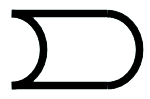
\includegraphics[width=1.1cm]{tablas-images/archi/business/archi_event.png}
& B-08 Evento de Negocio
& Conductual
& Suceso que desencadena o afecta la ejecución de procesos o funciones dentro del negocio.
& ArchiMate 3.x \\
\hline


\includegraphics[width=1.1cm]{tablas-images/archi/business/archi_service.png}
& B-09 Servicio de Negocio
& Conductual (externo)
& Funcionalidad ofrecida por el negocio a actores externos o internos.
& ArchiMate 3.x \\
\hline

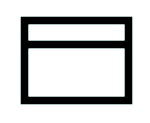
\includegraphics[width=1.1cm]{tablas-images/archi/business/archi_object.png}
& B-10 Objeto de Negocio
& Estructural pasivo
& Elemento de información relevante dentro del dominio del negocio.
& ArchiMate 3.x \\
\hline

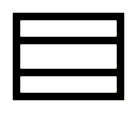
\includegraphics[width=1.1cm]{tablas-images/archi/business/archi_contract.png}
& B-11 Contrato
& Estructural pasivo
& Acuerdo formal que define derechos, obligaciones y condiciones entre partes.
& ArchiMate 3.x \\
\hline

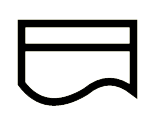
\includegraphics[width=1.1cm]{tablas-images/archi/business/archi_representation.png}
& B-12 Representación
& Estructural pasivo
& Forma perceptible o materializada de un objeto de negocio.
& ArchiMate 3.x \\
\hline

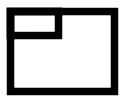
\includegraphics[width=1.1cm]{tablas-images/archi/business/archi_product.png}
& B-13 Producto
& Estructural compuesto
& Conjunto de servicios y valor ofrecido por el negocio a sus clientes.
& ArchiMate 3.x \\
\hline

% ==========================================================
% ======== EXTENSIONES PROPUESTAS EN NDTI ==================
% ==========================================================

\hline
\multicolumn{5}{|c|}{\textbf{Extensiones propuestas por el proyecto}} \\
\hline


\includegraphics[width=1.1cm]{tablas-images/archi/business/ndti_start.png}
& B-14 Inicio de flujo
& Evento
& Elemento que indica el punto de inicio de un proceso de negocio. Representa el momento en que se desencadena la ejecución de un flujo de actividades.
& Google Fonts \\
\hline


\includegraphics[width=1.1cm]{tablas-images/archi/business/ndti_end.png}
& B-15 Fin de flujo
& Evento
& Elemento que indica la finalización de un proceso de negocio, representando el término de un flujo de actividades.
& Google Fonts \\
\hline


\includegraphics[width=1.1cm]{tablas-images/archi/business/ndti_lane.png}
& B-16 Carril (Lane)
& Elemento estructural
& División visual de un proceso de negocio que organiza las actividades según actores, roles o áreas responsables, permitiendo una mejor comprensión de la asignación de responsabilidades.
& Propuesta estudiantes \\
\hline


\includegraphics[width=1.1cm]{tablas-images/archi/business/ndti_gateway.png}
& B-17 Ramificación / Decisión
& Elemento conductual
& Nodo que permite dividir el flujo de un proceso en múltiples caminos según condiciones definidas, representando decisiones dentro del proceso de negocio.
& Google Fonts \\
\hline


\includegraphics[width=1.1cm]{tablas-images/archi/business/ndti_andor.png}
& B-18 Operador lógico (AND/OR)
& Elemento conductual
& Elemento que permite representar condiciones lógicas dentro de un flujo de negocio, indicando ejecución paralela (AND) o selección alternativa (OR).
& Google Fonts \\
\hline

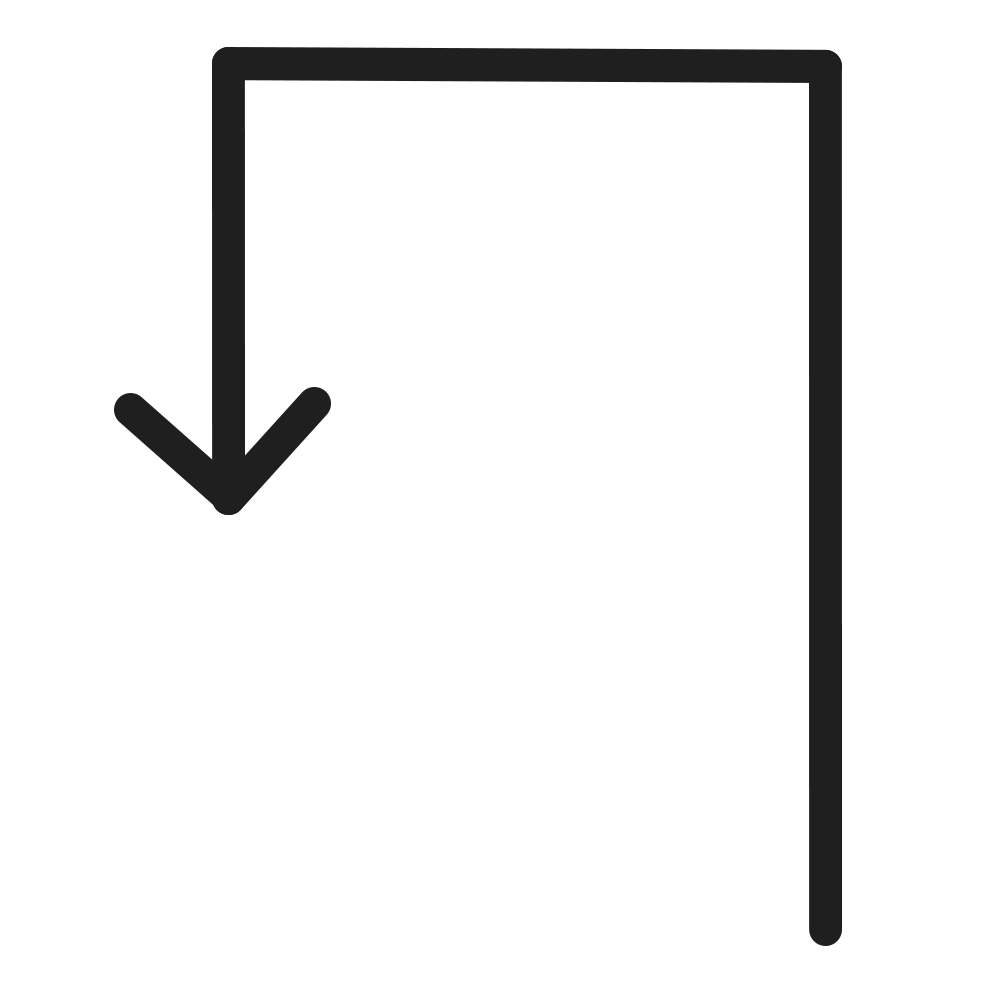
\includegraphics[width=1.1cm]{tablas-images/archi/business/ndti_loop.png}
& B-19 Bucle
& Elemento conductual
& Representación de la repetición de una o varias actividades dentro de un proceso de negocio hasta que se cumpla una condición específica.
& Google Fonts \\
\hline


\includegraphics[width=1.1cm]{tablas-images/archi/business/ndti_parallel.png}
& B-20 Paralelización
& Elemento conductual
& Nodo que permite la ejecución simultánea de múltiples actividades dentro de un proceso de negocio, facilitando la representación de flujos concurrentes.
& Google Fonts \\
\hline

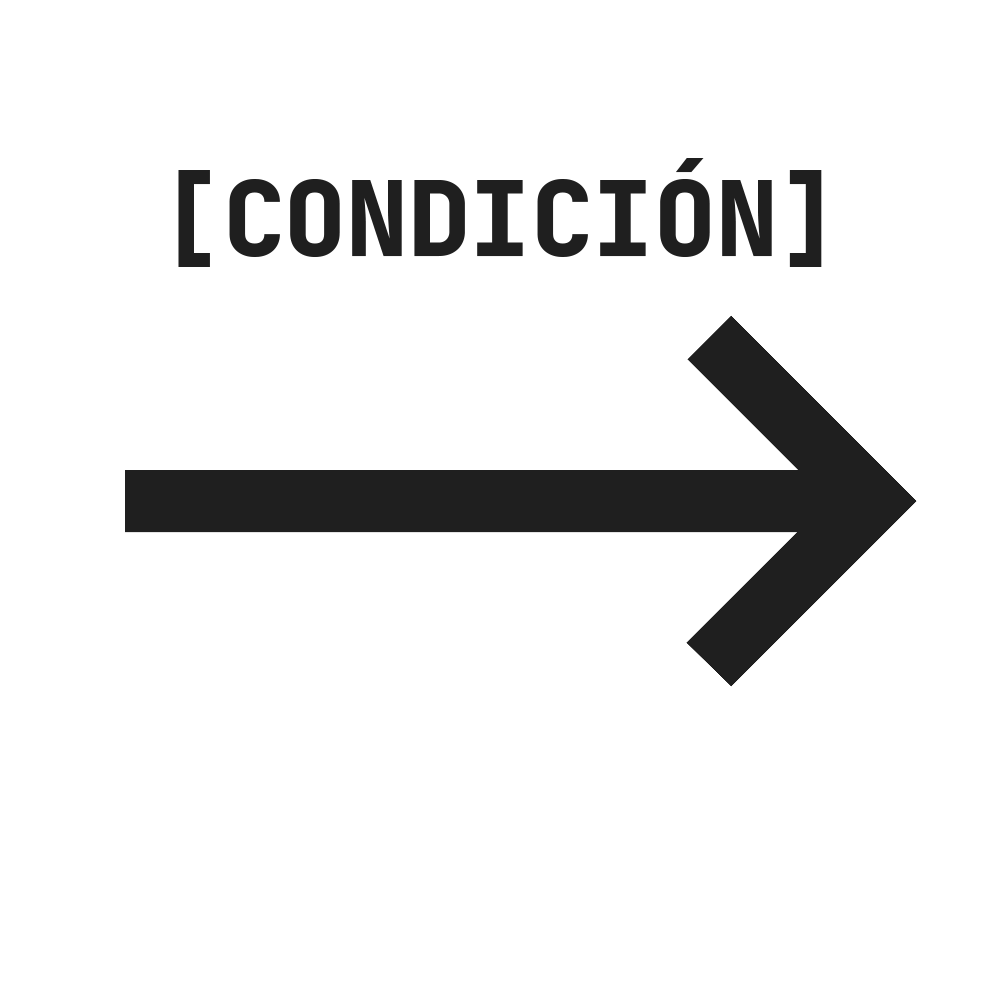
\includegraphics[width=1.1cm]{tablas-images/archi/business/ndti_condition.png}
& B-21 Condicional
& Elemento auxiliar
& Anotación que especifica la condición lógica necesaria para que un flujo o actividad sea ejecutado dentro del proceso de negocio.
& Google Fonts \\
\hline


\includegraphics[width=1.1cm]{tablas-images/archi/business/ndti_multievent.png}
& B-22 Evento múltiple
& Evento
& Representa la ocurrencia de múltiples eventos que pueden desencadenar o afectar el flujo de un proceso de negocio.
& Google Fonts \\
\hline


\includegraphics[width=1.1cm]{tablas-images/archi/business/ndti_frequency.png}
& B-23 Frecuencia
& Elemento auxiliar
& Elemento que permite indicar la periodicidad o recurrencia de una actividad dentro de un proceso de negocio (por ejemplo: diario, semanal, por demanda).
& Google Fonts \\
\hline

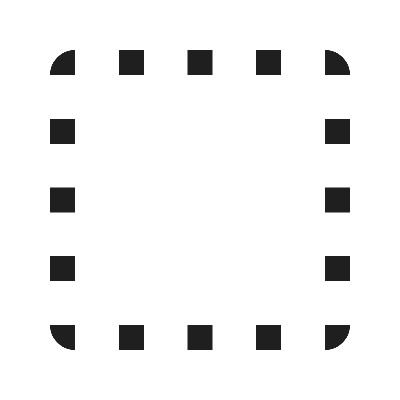
\includegraphics[width=1.1cm]{tablas-images/archi/business/ndti_independent.png}
& B-24 Acción independiente
& Conductual
& Actividad de negocio que puede ejecutarse de manera autónoma sin depender directamente de otras acciones dentro del flujo.
& Google Fonts \\
\hline


\includegraphics[width=1.1cm]{tablas-images/archi/business/ndti_recurrent.png}
& B-25 Acción recurrente
& Conductual
& Actividad de negocio que se ejecuta de manera repetitiva dentro de un proceso, generalmente asociada a condiciones o ciclos definidos.
& Google Fonts \\
\hline


\includegraphics[width=1.1cm]{tablas-images/archi/business/ndti_note.png}
& B-26 Anotación de texto
& Elemento auxiliar
& Elemento utilizado para agregar información descriptiva o aclaratoria dentro del modelo sin afectar su semántica estructural o conductual.
& Google Fonts \\
\hline

\end{longtable}


\subsubsection{Requisitos no-funcionales}
\noindent
Según \cite{4384163} un requisito no-funcional es un atributo o una restricción de un sistema. A continuación se definen los requisitos no-funcionales para la \textit{Grid App}.
\input{tablas-images/pruebas/requisitosNoFuncionales.tex}

\subsection{Pruebas}
\noindent
Para esta sección, se definen las pruebas y los pasos para ejecutar cada prueba.
\input{tablas-images/pruebas/pruebas.tex}

\subsection{Casos de uso}
\noindent
Luego de tener las pruebas que se van a ejecutar al sistema de la \textit{Grid App} ya definidas, se procede con la creación de un caso de uso por cada prueba. Esto tiene 3 motivaciones en este trabajo; (1) Mostrar la utilidad del sistema para un usuario ficticio, (2) Limitar el alcance del prototipo a unos casos de uso concretos y (3) Guiar el desarrollo hacia situaciones reales y la utilidad para los \textit{stakeholders}.

A continuación se definen los casos de uso:

\subsubsection{Caso 1: \textit{Montecarlo} para $\pi$}
\noindent
\begin{itemize}
    \item \textbf{Descripción:} En un laboratorio de investigación financiera, los analistas necesitan valuar instrumentos derivados complejos utilizando métodos \textit{Montecarlo} que requieren cientos de simulaciones. La infraestructura HTCondor distribuye estos cálculos estadísticos masivos a través de múltiples nodos, donde cada trabajo ejecuta una porción de las simulaciones para calcular aproximaciones de $\pi$ como prototipo, y luego consolida los resultados para obtener una mejor estimación que valide la confiabilidad del sistema en modelos de riesgo financiero.
    \item \textbf{Escenario de prueba relacionado:} ESC-01
\end{itemize}

\subsubsection{Caso 2: Conteo de números primos}
\noindent
\begin{itemize}
    \item \textbf{Descripción:} Un centro de criptografía debe analizar la distribución de números primos en intervalos grandes para evaluar la seguridad de algoritmos de encriptación RSA. HTCondor divide automáticamente estos rangos numéricos en sub intervalos que distribuye entre nodos heterogéneos, permitiendo el conteo concurrente de primos que demuestra la capacidad del sistema para manejar cargas computacionales intensivas.
    \item \textbf{Escenario de prueba relacionado:} ESC-02
\end{itemize}

\subsubsection{Caso 3: \textit{Quicksort} Paralelo}
\noindent
\begin{itemize}
    \item \textbf{Descripción:} Un instituto de genómica requiere ordenar cantidades enormes de datos de secuencias de ADN para identificar patrones de mutaciones genéticas. El algoritmo de \textit{quicksort} paralelo implementado con \MPI aprovechar los recursos agregados de memoria y procesamiento de múltiples máquinas bajo HTCondor, validando la capacidad de la infraestructura para coordinar trabajos que necesitan comunicación entre procesos (\IPC) en aplicaciones científicas.
    \item \textbf{Escenario de prueba relacionado:} ESC-03
\end{itemize}

\section{Modelado del sistema en Archimate}
\noindent
ArchiMate es un lenguaje de modelado estándar, abierto e independiente de~\textit{The Open Group} que permite representar de manera estructurada y general las diferentes capas de una arquitectura empresarial: negocio, aplicación y tecnología \citep{josey2016introduction}. Esto permite tener una visión integrada que facilita la comunicación entre los distintos actores de un negocio y que muestre cómo los procesos, los sistemas de información y la infraestructura tecnológica se relacionan entre sí.
A su vez, Archi es un Software que permite realizar diagramas de ArchiMate de forma sencilla y fue el Software elegido por el equipo de este proyecto para modelar las relaciones del proyecto con el negocio y varios elementos más. Archi permite dividir los modelos en vistas, que facilitan la organización y hacen más sencilla la labor de ampliar ciertos elementos o modelos importantes.

Cabe recalcar que algunos de los elementos como la misión y la visión no se muestran de forma completa en las vistas debido a su gran extensión textual. Sin embargo, con el fin de mostrar información completa, se mencionan y describen a continuación.

\begin{itemize}
    \item \textbf{Misión:} El Grupo de Investigación en Redes, Información y Distribución - GRID tiene como objetivo principal la realización de proyectos de investigación en temas relacionados principalmente con soluciones informáticas en Infraestructura Computacional, la Ingeniería de Software, el Análisis de Datos y la Informática Educativa. Hacer investigación en los temas mencionados, así como realizar proyectos interdisciplinarios deberá redundar en conocimientos frescos y la adopción de nuevas tecnologías que contribuyan al desarrollo académico del Programa Ingeniería de Sistemas y Computación, la Maestría en Ingeniería, y la Maestría y el Doctorado en Educación de la Universidad del Quindío. Luego de 10 años de existencia, de haber superado exitosamente los procesos de formación a nivel doctoral y de maestría de nuestros integrantes y de haber logrado la categoría C en el escalafón nacional de Ministerio de Ciencia, Tecnología e Innovación, nuestros esfuerzos estarán centrados en: (1) la formación de estudiantes a nivel de pregrado, maestría y doctorado; (2) fortalecer los lazos de amistad y colaboración con investigadores y grupos de investigación a nivel nacional e internacional; (3) la realización de proyectos de investigación y desarrollo de productos de nuevo conocimiento que busquen dar solución a problemas de la sociedad; y (4) aumentar la visibilidad del grupo y mejorar la categoría en el escalafón de MinCiencias.
    \item \textbf{Visión:} Para el año 2025, el Grupo de Investigación en Redes, Información y Distribución - GRID de la Facultad de Ingeniería de la Universidad del Quindío será un grupo consolidado y reconocido en la más alta categoría del escalafón nacional del Ministerio de Ciencia Tecnología e Innovación, que a través de sus aportes sea tenido en cuenta en la toma de decisiones a nivel regional y nacional; y con reconocimiento internacional mediante la realización de trabajos en colaboración con investigadores de otras universidades nacionales y extranjeras. Misión: Somos un grupo de profesores universitarios dedicados a realizar investigación en áreas tecnológicas orientadas a facilitar procesos y resolver problemas de la comunidad académica, de la sociedad que nos rodea y del sector productivo, mediante la adaptación de tecnologías o el desarrollo de soluciones informáticas en Infraestructura Computacional, la Ingeniería de Software, el Análisis de Datos y la Informática Educativa que constituyan un aporte al desarrollo social, económico y tecnológico de la región y el país.
    \item \textbf{Objetivo estratégico 1:} Realizar proyectos de investigación en los temas relacionados con las áreas de interés del grupo, así como proyectos interdisciplinarios que permitan la adopción de conocimientos y nuevas tecnologías que contribuyan al desarrollo de la región, del país y de la comunidad académica mundial.
    \item \textbf{Objetivo estratégico 2:} Establecer contactos con otros grupos de investigación interesados en temáticas similares, pertenecientes a otras instituciones de educación superior, tanto a nivel nacional como internacional.
    \item \textbf{Objetivo estratégico 3:} Impulsar la investigación dentro de la Universidad del Quindío y la Facultad de Ingeniería, particularmente en el programa Ingeniería de Sistemas y Computación, el programa de Maestría en Ingeniería, y los programas de Maestría y Doctorado en Educación.
    \item \textbf{Objetivo estratégico 4:} Establecer una comunidad académica con la participación de estudiantes de pregrado y posgrado, profesores y jóvenes investigadores.
\end{itemize}

\subsection{Vista de misión, visión y objetivos}
\noindent
        En la Figura \ref{fig:archiMVOView} se muestra las relaciones entre la misión, la visión y los objetivos estratégicos del negocio. Además, se muestran los ámbitos clave en los que se enfoca el negocio para cumplir con sus objetivos estratégicos. Esta última información se tomó de conversaciones informales con el representante del negocio para este proyecto, quien manifestó que estos son los enfoques que se le debe dar al proyecto y están dados por la organización a la que está adscrito el negocio, que para nuestro caso específico es el Grupo \GRID.\begin{figure}[H]
	\centering
	\includegraphics[scale=0.15]{tablas-images/archi/Mission-Values-Vision View.jpg}
	\caption{Vista de misión, visión y objetivos}
    \label{fig:archiMVOView}
\end{figure}

\subsection{Vista de mapa de valor estratégico}
\noindent
En la Figura \ref{fig:archiSVMView} se muestra el valor estratégico del negocio desde distintas perspectivas y su descomposición hacia otros valores más concretos. Todo esto con el fin de conocer que perspectivas son de más interés para el negocio y cuáles valores componen dichas perspectivas. Esto ocurre en capa de motivación, por lo que estos valores estratégicos identificados servirán como los principios orientadores de la estrategia del negocio.

\begin{figure}[H]
	\centering
	\includegraphics[scale=0.15]{tablas-images/archi/Strategic Value Map View.jpg}
	\caption{Vista de mapa de valor estratégico}
    \label{fig:archiSVMView}
\end{figure}

\subsection{Vista de objetivos}
\noindent
En la Figura \ref{fig:archiGoalsView} se muestra un desglose completo de los objetivos del negocio. Para este fin se usó una variación de una estrategia conocida como 5W, que usa cinco preguntas para obtener información completa sobre un elemento. Estas preguntas son: ¿Quién?, ¿Qué?, ¿Cuándo?, ¿Dónde? Y ¿Por qué? \citep{5WAmitava}. Para el desglose de los objetivos del negocio en esta vista del modelo se hizo necesarias solo cuatro preguntas como se muestra en la Figura \ref{fig:archiGoalsView}. Así, podemos ver como está compuesta la motivación del negocio y los elementos que están en torno a los objetivos estratégicos.

\begin{figure}[H]
	\centering
	\includegraphics[scale=0.12]{tablas-images/archi/Goals View.jpg}
	\caption{Vista de objetivos}
    \label{fig:archiGoalsView}
\end{figure}

\subsection{Vista de servicio de negocio}
\noindent
En la Figura \ref{fig:archiBSView} se muestra la estructura del servicio de negocio que el proyecto relatado en este documento buscar intervenir, desde los objetivos estratégicos en cuanto a motivación hasta los componentes de aplicación, pasando por los servicios de aplicación y el servicio de negocio con una estructura mínima. Cabe recalcar que los nombres en inglés de algunos componentes corresponden a nombres propios que se le asignaron al componente

\begin{figure}[H]
	\centering
	\includegraphics[scale=0.13]{tablas-images/archi/Business Service View.jpg}
	\caption{Vista de servicio de negocio}
    \label{fig:archiBSView}
\end{figure}

\subsection{Vista de aplicación}
\noindent
En la Figura \ref{fig:archiAppView} se muestran de forma general, las características y procesos de las aplicaciones que componen la solución, además de la comunicación entre dichas aplicaciones y la información de intercambio. Sin embargo, la vista que nos ofrece ArchiMate en capa de aplicación puede ser un poco limitada cuando el objetivo es describir a detalle la forma en que funciona cada componente de la aplicación y del sistema en general. Por lo que se decide complementar este modelo con otros diagramas usando otros lenguajes de modelado un poco más adelante.

\begin{figure}[H]
	\centering
	\includegraphics[scale=0.12]{tablas-images/archi/Application View.jpg}
	\caption{Vista de aplicación}
    \label{fig:archiAppView}
\end{figure}

\subsection{Vista de infraestructura}
\noindent
En la Figura \ref{fig:archiInfrastructureView} se muestran de forma general, las características de los nodos de la infraestructura que componen la solución, además de las relaciones entre dichos nodos y su relación con las aplicaciones que corren en ellos. Sin embargo, al igual que pasa en la capa de aplicación, la vista que nos ofrece ArchiMate en capa de infraestructura puede ser un poco limitada cuando el objetivo es describir a detalle la forma en que funciona cada nodo de la infraestructura y su comunicación física. Por lo que se decide complementar este modelo con otros diagramas usando otros lenguajes de modelado un poco más adelante.

\begin{figure}[H]
	\centering
	\includegraphics[scale=0.103]{tablas-images/archi/Infrastructure View.jpg}
	\caption{Vista de infraestructura}
    \label{fig:archiInfrastructureView}
\end{figure}

\subsection{Vista por capas}
\noindent
El último modelo de ArchiMate que compone la solución es el mostrado en la Figura \ref{fig:archiLayeredView} en donde se unen de forma general los demás modelos mostrados anteriormente y se muestran sus relaciones a alto nivel. Todo esto con el fin de dar una visión general de las capas que componen la solución y así tener una idea global de la forma en que cada componente se comunica con los demás.

\begin{figure}[H]
	\centering
	\includegraphics[scale=0.125]{tablas-images/archi/Layered View.jpg}
	\caption{Vista por capas}
    \label{fig:archiLayeredView}
\end{figure}

\section{Modelado del software con el modelo C4}
\noindent
El modelo C4 es una herramienta que ayuda a los equipos de desarrollo de software a describir y comunicar la arquitectura del software a varios niveles de detalle. De forma general el modelo C4 tiene cuatro niveles, cada una con mayor nivel de detalle que la anterior. Para el caso de uso de este proyecto se optó por usar los tres primeros niveles, ya que se considera que el último nivel no da demasiado detalle visual para representar las interacciones en el ámbito de código, por lo que para este fin se usará otro diagrama presentado más adelante.

\subsection{Nivel 1: Diagrama de contexto del sistema}
\noindent
El diagrama de contexto del sistema muestra de forma muy general y a muy alto nivel la solución que se propone. Lo que permite una visión global y generalizada, útil para comprender rápidamente los elementos de la solución.

En la Figura \ref{fig:C4Nivel1} se muestra los elementos principales de la arquitectura, los nombres de dichos elementos, la interacción entre ellos y la comunicación que realizan con el usuario. Como se puede apreciar en el diagrama, el sistema está compuesto de tres aplicaciones y los tres universos de HTCondor que componen la solución. Cabe aclarar que la aplicación denominada \textit{Tablero App} ya estaba implementada en un clúster antes del inicio de este proyecto. Sin embargo, se adiciona a la arquitectura de la solución, ya que se hizo un esfuerzo para adaptar está en todos los clústeres Vanilla que componen la solución.

\begin{figure}[H]
	\centering
	\includegraphics[scale=0.1]{tablas-images/C4/Diagramas HTCondor-Nivel 1.drawio.png}
	\caption{Diagrama de contexto del sistema}
    \label{fig:C4Nivel1}
\end{figure}

\subsection{Nivel 2: Diagrama de contenedores}
\noindent
El diagrama de contenedores muestra los elementos básicos dentro de cada sistema de Software. Lo que permite ir un poco más allá y entender como funciona cada sistema de software por dentro y como interactúa con el resto de contenedores.

En la Figura \ref{fig:C4Nivel2} se muestran los contenedores principales de la arquitectura, los nombres de dichos contenedores, la interacción entre ellos y la comunicación que realizan con el usuario. Como se puede apreciar en el diagrama, el sistema está compuesto por: (1) Un \textit{backend} que cumple dos funciones principales; la primera es renderizar las plantillas que se le van a mostrar al usuario pues estás contienen información dinámica que debe ser consultada y establecida por el servidor, la segunda es realizar toda la lógica de la aplicación como despertar otros procesos o construir los archivos maestros de HTCondor. Se optó por este enfoque en el diseño para propender por la simplicidad de la aplicación y su fácil portabilidad y despliegue en diferentes tipos de entornos. En el Apéndice XX se muestra el código de los componentes y la estructura de los directorios de este componente. (2) Un directorio dentro del sistema de archivos del equipo que sirve la aplicación \textit{Grid App} en donde se almacenan los resultados de los trabajos. (3) Los universos de HTCondor que se propusieron implementar en este proyecto, estos son, Parallel y Grid, pues el Vanilla ya estaba implementado y (4) una aplicación llamada \textit{Cluster Info App} en cada clúster de HTCondor que recoge métricas básicas y las expone en formato \JSON a través de una \API.

\begin{figure}[H]
	\centering
	\includegraphics[scale=0.1]{tablas-images/C4/Diagramas HTCondor-Nivel 2.drawio.png}
	\caption{Diagrama de contenedores}
    \label{fig:C4Nivel2}
\end{figure}

\subsection{Nivel 3: Diagrama de componentes}
\noindent
El diagrama de componentes muestra los elementos básicos dentro de cada contenedor. Lo que permite ir aún más allá y entender de forma profunda como están compuestos los elementos del Software y que realizan a nivel interno. Para este nivel de granularidad se decide dividir el diagrama de componentes en distintas partes. Con el fin de hacer más sencilla su lectura y comprensión.

\subsubsection{Universo \textit{Vanilla}}
\noindent
En la Figura \ref{fig:C4Nivel3Vanilla} se muestran los componentes principales de la arquitectura del universo Vanilla en HTCondor. Además, se pueden apreciar los distintos procesos que sigue un trabajo desde su envío hasta la recepción de sus resultados.

\begin{figure}[H]
	\centering
	\includegraphics[scale=0.09]{tablas-images/C4/Diagramas HTCondor-Nivel 3 - Vanilla.drawio.png}
	\caption{Diagrama de componentes para el universo Vanilla}
    \label{fig:C4Nivel3Vanilla}
\end{figure}

\subsubsection{Universo \textit{Parallel}}
\noindent
En la Figura \ref{fig:C4Nivel3Parallel} se muestran los componentes principales de la arquitectura del universo Parallel en HTCondor. Además, se pueden apreciar los distintos procesos que sigue un trabajo desde su envío hasta la recepción de sus resultados. Es importante notar que ls comunicación y los componentes funcionan exactamente de la misma forma que en el universo Vanilla, con la unica diferencia que aquí, los trabajo se comunican a través de \MPI.

\begin{figure}[H]
	\centering
	\includegraphics[scale=0.09]{tablas-images/C4/Diagramas HTCondor-Nivel 3 - Parallel.drawio.png}
	\caption{Diagrama de componentes para el universo Parallel}
    \label{fig:C4Nivel3Parallel}
\end{figure}

\subsubsection{Universo \textit{Grid}}
\noindent
En la Figura \ref{fig:C4Nivel3Grid} se muestran los componentes principales de la arquitectura del universo Grid en HTCondor. Como se puede apreciar en el digrama este universo actua como un intermediario entre el usuario y el clúster que va a ejecutar su trabajo, permitiendo así interconectar multiples clústeres, donde reside el valor de este universo.

\begin{figure}[H]
	\centering
	\includegraphics[scale=0.1]{tablas-images/C4/Diagramas HTCondor-Nivel 3 - Grid.drawio.png}
	\caption{Diagrama de componentes para el universo Grid}
    \label{fig:C4Nivel3Grid}
\end{figure}

\subsubsection{Aplicaciones de Software}
\noindent
En la Figura \ref{fig:C4Nivel3Apps} se muestran los componentes principales de las aplicaciones que integran el sistema. Como se puede evidenciar en el diagrama, hay dos aplicaciones principales que conforman este sistema. La primera es la aplicación central \textit{Grid App} que ayuda a abstraer la complejidad de HTCondor con una interfaz \textit{web} más amigable, además, es la encargada de enviar los trabajos y recoger los resultados. La segunda es la \textit{Cluster Info App} que ayuda a exponer métricas de cada clúster, permitiendo así a la aplicación central obtener datos reales de cada clúster y permitir al usuario elegir el clúster con métricas más favorables para su caso de uso. Es importante aclarar que la aplicación \textit{Tablero App} también está disponible y funcionando en algunos de los clústeres que componen la solución. Sin embargo, dado que su única labor es mostrar métricas detalladas del clúster, se opta por no agregarlo al diagrama por dos razones: (1) para reducir su complejidad y (2) porque el desarrollo de esta aplicación no es resultado del desarrollo de este proyecto.

\begin{figure}[H]
	\centering
	\includegraphics[scale=0.09]{tablas-images/C4/Diagramas HTCondor-Nivel 3 - Apps.drawio.png}
	\caption{Diagrama de componentes para las aplicaciones que componen el sistema}
    \label{fig:C4Nivel3Apps}
\end{figure}

\section{Modelado de secuencia con UML}
\UML es un lenguaje de modelado orientado a múltiples enfoques como la secuencia de eventos y la estructura de las clases \citep{10.1145/1125944.1125949}. Para el caso de este proyecto se usará para describir de forma concreta y estructurada la secuencia que siguen los componentes del Software en cada momento, así como las alternativas que toma el programa con base en la información disponible. De igual forma, se usará este lenguaje para modelar la estructura de las clases que transportan información a través del programa. Cabe aclarar que el sistema no se diseña con una orientación a objetos estricta. Sin embargo su forma principal de intercambio de información es a través de \JSON. Por lo que se hace necesario conocer y describir la forma de los objetos que se intercambian.

\subsection{Diagrama de secuencia}
\noindent
En la Figura \ref{fig:UMLSecuencia} se muestran los procesos y llamados que se ejecutan en cada paso del sistema, desde las rutas que se visitan hasta la información que se transfiere en cada momento. Es importante añadir que la información de transferencia entre cada sistema de software es meramente ilustrativa y para dar mayor profundidad a dicha información, debe complementarse con el diagrama de clases presentado en la sección siguiente y el código de la aplicación presentado en el Apéndice XX.

\begin{figure}[H]
	\centering
	\includegraphics[scale=0.11]{tablas-images/UML/Diagramas HTCondor-Secuencia.drawio.png}
	\caption{Diagrama de secuencia para el sistema}
    \label{fig:UMLSecuencia}
\end{figure}

\subsection{Diagrama de clases}
\noindent
En la Figura \ref{fig:UMLClases} se muestra la composición de las clases en las que se basan los objetos que permiten intercambiar información a través de los sistemas. Debido a que el diseño no fue orientado a objetos, este diagrama solo pretende mostrar los elementos de información que intercambia el sistema y no pretende modelar la arquitectura general de los sistemas de software.

\begin{figure}[H]
	\centering
	\includegraphics[scale=0.1]{tablas-images/UML/Diagramas HTCondor-Objetos.drawio.png}
	\caption{Diagrama de clases para el sistema}
    \label{fig:UMLClases}
\end{figure}

\section{Modelado de infraestructura con modelos personalizados}
Después de conocer como está compuesto el sistema de forma transversal con ArchiMate y en cuanto a software con C4 y \UML, se hace necesario un modelado más profundo de la infraestructura física y de red que compone la solución. Esto debido a que ArchiMate no da la profundidad necesaria para modelar esta clase de elementos, por lo que se opta por otras opciones con el fin de dar más profundidad al diseño y más claridad al lector sobre los elementos que componen la solución.

A pesar de esto, el equipo del proyecto no halló ningún lenguaje de modelado ni sistema formal que se armonizara con la clase de modelado de infraestructura que se pretende realizar. Por lo que se opta por usar una herramienta de modelado llamada draw.io y figuras genéricas con información complementaria que permiten tener una idea general de la infraestructura que subyace la solución.

\subsection{Modelo de infraestructura física}
\noindent
En la Figura \ref{fig:Fisica} se muestran los componentes de hardware principales que componen la solución. A su vez, se presentan las conexiones eléctricas que tiene cada elemento. Esto con el fin de mostrar la forma en que están conectados a la red eléctrica los componentes, ya que su conexión no es trivial y se hace necesaria documentación especializada que muestre este tipo de elementos.

\begin{figure}[H]
	\centering
	\includegraphics[scale=0.1]{tablas-images/personalizado/Diagramas HTCondor-Fisica.drawio.png}
	\caption{Modelo de infraestructura física}
    \label{fig:Fisica}
\end{figure}

\subsection{Modelo de enlace de datos}
\noindent
En la Figura \ref{fig:Enlace} se muestran las conexiones de red que tiene cada elemento. Esto con el fin de mostrar la forma en que están conectados los componentes a la red y a Internet, ya que su conexión no es trivial y se hace necesaria documentación especializada que muestre estás conexiones.

\begin{figure}[H]
	\centering
	\includegraphics[scale=0.1]{tablas-images/personalizado/Diagramas HTCondor-Enlace.drawio.png}
	\caption{Modelo de enlace de datos}
    \label{fig:Enlace}
\end{figure}

\subsection{Modelo de roles}
\noindent
Después de conocer como están conectados los elementos de infraestructura a nivel eléctrico y de red, se hace necesario plasmar la forma en que están conectados los elementos de forma lógica, que es la forma en que se comunican los elementos en el diseño de la solución. Además, se hace necesario mostrar los roles de HTCondor que ocupa cada elemento en su clúster. En la Figura \ref{fig:Roles} se plasman estos aspectos.

\begin{figure}[H]
	\centering
	\includegraphics[scale=0.088]{tablas-images/personalizado/Diagramas HTCondor-Roles.drawio.png}
	\caption{Modelo de roles}
    \label{fig:Roles}
\end{figure}